% by Wolfgang
% Not the final structure 
% not yet proof read 
% early colletion of topics
\section{Introduction} 
We have seen impressive improvements in the last years in the field of artificial intelligence (AI). Machines are able to detect faces in pictures (e.g. Facebook) and even recognizance the people in them. We have even seen, that are able machines to name any kind of object in pictures and produce descriptions for those (Google paper). Machines can also translate speech to text (e.g Siri) and play Atari Games better then any human (DeepMind Atari Paper). But all of these have one thing in common. This are all tasks that have a clear goal. There is only one solution to the given problem. Whether it is a high score in a game or the label apple in the picture with an apple. It is often thought that this is where it ends. Machines are never going to be creative! Machines can some day get better than any human in 'logical' task, but besides this machines can be creative or inventive. 
%Add references

According to a popular theory of mind (Computational theory of mind) 
%recherche
the human cognition is nothing more then a information processing machine. A complex and very efficient machine thou, but a machine. Following this idea we ask the question is there a possibility to implement aspects of creativity in an AI and what is needed to do so.   

We have chosen the music domain for that. We implemented a program that is able to create new music after it has heard other music. This   work shows how we did it and what this means for the question, weather a machine is able to be creative. It is still open whether this is to be considers creative. 

\subsection{The music domain}
We have chosen the music domain for several reason. First it is an area that enables creativity, there is a whole culture around music creation and playing music. Also creativity can be applied in any area (think about the creative problem solving) we wanted to work is a domain that claims to only be solvable with creativity. 

Second music has a representation on many different levels, as well as human cognition has. On the basic layer sound is moving particles is a wave, if the wave is constant we talk about tones. Music deals with tones on a scale. Starting at one root tone you built the tonality in a hierarchical fashion. At this layer of representation we normally start talking about music. It is clear that we already make some assumptions on how we perceive sound and what mid sound good. Normally in western music we just consider the Dur tonalities, and we will so in this work. 

The next layer are tones in the tonality ordered to a sequence. This layers describes what tones are played after another and what tones are played at the same time, in the music domain we normally talk of melody and harmony. We choose to work on this layer of symbolic representation. But there are even higher layers. There are pieces of music and whole concerts with each a theme or a story and there are even artists with different styles.

The interesting part about this is that all of this layers also are processed in a different way by humans. While creating (or just listening to music) all these layers are combined. But also the single layers a topic of inspection and one can be creative and inventive there as well. These properties are very useful for our exploration in computational creativity. This way we can focus an specific layers of the creative process and consider similar layers in the human cognition. We so are able to build cognitive inspired models that can also be discussed on the bases of information processing in the human brain. 

\subsection{The project approach}
The main idea of the project was to introduce a computer program that is able to produce music on it's own. This will give us insides in computational creativity.

To explore the possibilities we build a framework to test and explore computational accounts for music harmonization. This section will introduce  this framework, later we will refer to the parts in more detail.

Wile designing the framework the guiding principles where: molecularity and simplicity. The pipeline from input to output consisted of: Music representation - music piece (melody) - develop style - apply style to melody / harmonization - output music (e.g. musicxml)

Important to notice here is the differentiation between the 'creative' part and the harmonization part. We follow a two step process that consists of a style generation (creative) and the harmonization where this style is applied to the moldy (deterministic). This way we can explore different 'creative' modules in our abstract representation and then have the same predictive harmonization process in the end, to project it back into music space.

\subsection{System Architecture}
The system's pipeline is visualized in graphic (??). The left side shows the input to the system, that consists of a melody to harmonize  and a couple of known styles (see next chapter). All music that is input to the system is represented using our music representation using a sequences of vectors.

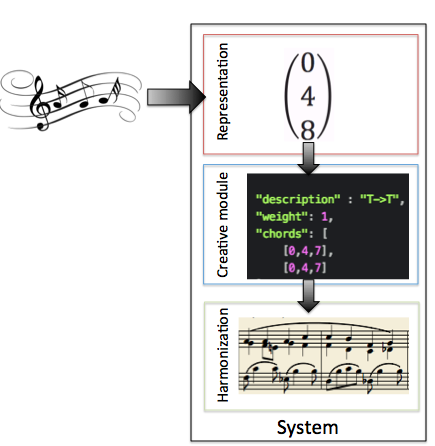
\includegraphics[scale=1]{Chapters/pic/sys_arch.png}

These styles are given by the user or generated out of other music or be the result of earlier runs and outcomes of the system.

The first part of the two step process is the creative part. Here the system creates a new style with given styles. This is where the creative algorithms are located. You can choose one of the creative modules and different styles to create different new styles. The new style is then in the next step used as a template to harmonize the given melody. This step in not to considered creative but make to be very predictive.

With splitting the process we are able to test different creative modules and produce just the style. We can then do both just visualize the style as the essence of the creative module or run the deterministic harmonization process with a melody to be able to listen to the creation. 